 % ------------------------------------------------
% SIGGRAPH Asia 2026 Technical Papers format
% ------------------------------------------------
\documentclass[acmtog,anonymous,review]{acmart}
\acmSubmissionID{1107}

% ------------------------------------------------
% Additional packages (ACM-approved)
% ------------------------------------------------
\usepackage{bm}
\usepackage{mathtools}
\usepackage{algorithm}
\usepackage{algorithmic}
\usepackage{enumitem}
\usepackage{tikz}
\usepackage{amsmath}
\usetikzlibrary{calc,fit,backgrounds,arrows.meta}

% ------------------------------------------------
% Algorithm environment
% ------------------------------------------------
\floatname{algorithm}{Algorithm}
\renewcommand{\algorithmicrequire}{\textbf{Input:}}
\renewcommand{\algorithmicensure}{\textbf{Output:}}

% ------------------------------------------------
% Math commands and operators
% ------------------------------------------------
\newcommand{\norm}[1]{\left\lVert #1 \right\rVert}
\newcommand{\abs}[1]{\left\lvert #1 \right\rvert}
\newcommand{\R}{\mathbb{R}}
\newcommand{\dd}{\,\mathrm{d}}
\newcommand{\T}{\mathsf{T}}
\newcommand{\xx}{\mathbf{x}}
\renewcommand{\gg}{\mathbf{g}}
\newcommand{\HH}{\mathbf{H}}
\newcommand{\yy}{\mathbf{y}}
\renewcommand{\vv}{\mathbf{v}}
\DeclareMathOperator{\conv}{conv}

\DeclareMathOperator*{\argmax}{arg\,max}
\DeclareMathOperator*{\argmin}{arg\,min}
\DeclareMathOperator*{\com}{com}
\DeclareMathOperator*{\mass}{mass}
\DeclareMathOperator{\diag}{diag}
\DeclareMathOperator{\tr}{tr}

\newtheorem{remark}{Remark}

% ------------------------------------------------
% Title (anonymous submission — no authors)
% ------------------------------------------------
\title{Continuous Collision Detection Trust Regions for Clothing Simulation}

\begin{document}

\begin{abstract}
We present a trust region technique for simulating clothing with barrier potentials.
Our method guarantees that each iteration of a nonlinear Gauss--Seidel solver maintains a collision free state.
While previous techniques have achieved this by limiting step sizes based on geometric proximity heuristics, we show that continuous collision detection can be used instead to greatly increase step sizes and, in turn, dramatically decrease computation time.
We define our trust regions as axis aligned bounding boxes that surround each vertex. By constraining each Gauss--Seidel vertex correction to remain in the respective box, we establish a worst-case collection of vertex/triangle and edge/edge interaction pairs that can occur over the time step.
These interactions occur through barrier potentials and continuous collision detection step size limitation.
Using this interaction information (together with elastic mesh connectivity) we color vertices that can be safely updated in parallel.
Notably, when vertices in a given color are being simultaneously updated (on different threads), our coloring guarantees that the continuous collision detection check involves only one moving vertex (since the remaining three vertices in the edge/edge or vertex/triangle pair are of different colors).
This reduces the notoriously rounding-sensitive cubic solve for potential collision to a simple linear solve.
We demonstrate the efficacy of our method in representative clothing simulation scenarios.
\end{abstract}

\maketitle

\section{Introduction}
The simulation of thin elastic materials in close contact is a ever present in physics based animation.
For example, virtual characters often wear a variety of layered garments (usually in the form of triangle meshes) that must collide with each other to prevent visual artifacts.
While elastic constitutive forces in the cloth naturally use the static structure of the mesh, collision forces utilize different portions of the mesh at different times and are generally much more challenging to resolve \cite{Baraff1998LargeSteps}.
Furthermore, the continuous collision detection (CCD) problem where each point/triangle and segment/segment mesh pair is prevented from colliding over the course of each time step is also required to guarantee a collision free state \cite{bridson2002cloth}.
In this problem, mesh vertices are assumed to follow linear trajectories over a time step, which reduces the determination of if and when a point/triangle or segment/segment pair will collide to examining their proximity at the roots of a cubic that lie in the time step interval.
This problem is both costly and sensitive to rounding errors \cite{brochu:2012:ccd,Wang:2022:FastRootParity}.
Despite these complications, cloth simulators must navigate these challenges when collision-free guarantees are required.\\
\\
Simulation techniques use a wide variety of models for the collision forces and for solving the CCD problem.
The most common collision forces are based on simple quadratic potential energy springs, but they are limited in their ability to prevent all collision \cite{chen2024xpbd}.
Incremental potential contact (IPC) techniques have shown that a singular potential can be used to better prevent collision \cite{li2020ipc}.
However, these require the addition of a CCD-informed line search to backtrack and prevent crossing the singularity.
Li et al. \shortcite{li2020ipc} create a hypothetical step direction using Newton's method and then examine the first time that a collision would occur between point/triangle and/or segment/segment pairs.
The step size is then uniformly truncated across all vertices based on this worst-case collision time.
Impulse-based techniques avoid issues associated with singular barrier potentials and instead iteratively resolve collision pairs by adding momentum conserving impulses one pair at a time \cite{bridson2002cloth}.
However, because each impulsive correction only considers one pair at at time, it can cause collision in neighboring pairs.
This is addressed by iterating over all pairs over and over, but it is not guaranteed to converge to a collision free state in practice.
Indeed large iteration counts for these techniques can lead to excessive run times.\\
\\
Recently, trust region techniques have been adopted that circumvent the need for the CCD check \cite{wu2020repulsion,chen2025ogc}.
In these approaches, each mesh vertex computes a safe radius that it is allowed to move within.
By conservatively examining the proximity between each point/triangle and edge/edge pair in the mesh (and assuming a collision free state), a safe step size can be determined for each vertex (e.g. less than half the minimum distance between the point/triangle and edge/edge pairs it is in).
Chen et al. \shortcite{chen2025ogc} use this idea is used with a barrier potential. 
They use the Vertex Block Descent (VBD) Gauss--Seidel technique \shortcite{chen2024vbd} and allow each vertex to move independently (within its trust region).
This avoids the problem of Li et al. \shortcite{li2020ipc} where step size is based on a distant/worst case colliding pair.
However, the safe radius can be overly small and convergence limiting in practice (e.g. consider regions of the mesh in close proximity, but with separating velocities).\\
\\
While the Gauss--Seidel nature of VBD allows for localized collision step limiting,  a coloring technique is needed for efficient parallel implementation \cite{chen2024xpbd,chen2024vbd}.
A greedy coloring of vertices based on elastic mesh and collision interactions is needed so that vertices in a given color do not interact (via elastic or collision forces).
However, this is costly with the introduction of the barrier potential.
As a vertex changes position during the Gauss-Seidel iteration, it will potentially cause barrier interactions between different point/triangle and edge/edge pairs.
When this happens, the coloring information needs to be updated, which is costly given the frequency with which this can occur.
Chen et al. \shortcite{chen2024vbd,chen2025ogc} avoid re-coloring based on new barrier interactions, however this degrades the iteration (from Gauss--Seidel) to the slower convergencing Jacobi iteration.
Chen et al. \shortcite{chen2024xpbd} preserve the Gauss--Seidel behavior but avoid this problem by using a simple quadratic spring barrier potential that changes once per time step (and therefore loses all collision-free guarantees).
\\
\\
We design a trust region technique that utilizes CCD to allow for larger step sizes and a natural vertex coloring that can be done efficiently.
Like Chen et al. \shortcite{chen2025ogc}, we use a barrier potential and Gauss--Seidel iteration to avoid the global step size limitation in Li et al. \shortcite{li2020ipc}.
However, by using CCD we remove the overly conservative per-vertex step size restrictions of Wu et al. and Chen et al. \shortcite{wu2020repulsion,chen2025ogc}.
To achieve this, we restrict vertices to move inside axis-aligned bounding boxes (AABBs) during the iterative update.
By restricting vertex motion in this way, edges and triangles move in predictable boxes created by their vertices.
We can then determine worst-case point/triangle and edge/edge interactions so that every vertex knows a super-set of collision pairs that its motion may effect over the update.
Because our barrier energy is also based on these pairs we then also know a super set of which pairs will effect the barrier potential (and therefore subsequent collision force interactions).
This gives us enough interaction information to create a vertex coloring that does not need to be redone until the vertex AABBs are allowed to change (subject to user control).
The added benefit of this coloring is that vertices in the same color do not interact through CCD, barrier potentials or elastic forces.
This means that point/triangle and edge/edge CCD checks associated with the a vertex update are done with only one moving vertex.
This reduces the rounding-sensitive cubic solve for collision times to a simple linear solve, dramatically reducing run-time, code complexity and rounding sensitivity.
We demonstrate that our CCD trust region technique guarantees a collision free state and dramatically improves run-time while allowing for larger step sizes in collision intensive scenarios.

\section{Related Work}

\paragraph{Incremental Potential Contact.}
Li et al.~\cite{li2020ipc} introduced Incremental Potential Contact
(IPC), a variational framework that guarantees intersection- and
inversion-free dynamics for deformable bodies through log-barrier
energies and continuous collision detection.
Ferguson et al.~\cite{ferguson2021ipc} extended IPC to rigid body
dynamics.
Ferguson et al.~\cite{ferguson2023highorder} further extended IPC to
high-order finite elements on curved meshes, mapping contact forces
between a linear collision proxy and the high-order representation.
Li et al.~\cite{li2021cipc} generalized the framework to
codimensional structures including shells, rods, and their coupling.
Lan et al.~\cite{lan2022abd} introduced affine body dynamics, which
relaxes rigidity to an affine motion model for orders-of-magnitude
speedups on stiff materials while preserving IPC's non-intersection
guarantees.
Huang et al.~\cite{huang2024gipc} proposed GIPC, a GPU-optimized
IPC solver that derives analytic eigensystems for the barrier
Hessian, avoiding numerical eigendecomposition and enabling
significant acceleration.
Huang et al.~\cite{huang2025stiffgipc} further introduced StiffGIPC,
combining a connectivity-enhanced multilevel preconditioner with
cubic strain-limiting energies for stiff membranes such as cloth,
achieving up to $10\times$ speedup over prior GPU IPC methods.
Li et al.~\cite{li2023subspace} combined subspace preconditioning
with GPU Jacobi iteration for cloth simulation, coupling IPC contact
handling with projective dynamics.

\paragraph{Collision detection and avoidance.}
Bridson et al.~\cite{bridson2002cloth} established the standard
continuous collision detection framework based on coplanarity tests
that we adopt for step filtering. 
Brochu et al.~\cite{brochu2012exact} showed that the underlying
cubic polynomial solver is vulnerable to rounding error, particularly
in near-planar configurations.
Ericson~\cite{ericson2004collision}
provides a comprehensive reference for bounding volume hierarchies
and swept AABB queries.
Wu et al.~\cite{wu2020repulsion} proposed a condition-based collision
avoidance method for cloth self-collisions, avoiding
explicit CCD.
Wang et al.~\cite{wang2021tightinclusion} introduced a large-scale
CCD benchmark and proposed the Tight-Inclusion algorithm, an
inclusion-based method that provides conservative, gap-free collision
detection with support for minimum separation.
Chen et al.~\cite{chen2025ogc} introduced offset geometric contact,
which enforces separation constraints via geometric offsets and
trust-region step filtering as an alternative to
CCD-based line search.

\paragraph{Optimization time integration.}
Gast et al.~\cite{gast2015optimization} formulated implicit time
integration as an optimization problem, enabling large stable time
steps for elasticity simulation. The incremental potential
formulation~\cite{li2020ipc} builds on this variational perspective,
and our solver inherits the same structure while replacing the global
minimization with coordinate-wise descent.

\paragraph{Position-based methods.}
Macklin et al.~\cite{macklin2016xpbd} introduced XPBD, extending
position-based dynamics to handle compliant constraints with implicit
time stepping. While efficient and widely adopted, XPBD solves a
compliance-regularized system whose solutions depend on iteration
count and do not converge to a physically consistent equilibrium.

\paragraph{Nonlinear Gauss--Seidel methods.}
Fratarcangeli et al.~\cite{fratarcangeli2016vivace} introduced a
parallel Gauss--Seidel method using randomized graph coloring for
soft body dynamics.
Chen et al.~\cite{chen2024vbd} proposed vertex block descent (VBD),
a vertex-level Gauss--Seidel method for the variational implicit
Euler problem that achieves unconditional stability and convergent
solutions with maximized parallelism.
Chen et al.~\cite{chen2024xpbd} applied a similar nonlinear
Gauss--Seidel strategy to quasistatic hyperelasticity, achieving
fast convergence without global linear solves.
Lan et al.~\cite{lan2025jgs2} proposed a GPU Jacobi/Gauss--Seidel
method that mitigates overshoot to achieve near second-order
convergence comparable to Newton's method. Our method extends these
ideas to the dynamic setting with contact, incorporating IPC barrier
energies, continuous collision detection, and a parallel batching
scheme based on conflict graph coloring.

\paragraph{Constitutive models.}
We use the corotated elastic energy of Stomakhin et
al.~\cite{stomakhin2012elasticity} for membrane stretching and the
discrete shell bending model of Grinspun et
al.~\cite{grinspun2003discrete}. Both are standard choices for thin
shell simulation.

\section{Overview}
\label{sec:gs_ipc}
We represent our thin elastic materials with triangle meshes.
We use $\mathbf{x}^n\in\mathbb{R}^{3N_V}$ to denote the array of mesh vertex positions at time $t^n$ (where $N_V$ is the number of vertices in the mesh).
$\mathbf{v}^n\in\mathbb{R}^{3N_V}$ represents the array of mesh vertex velocities.
We use the notation $\mathbf{x}^n_i\in\mathbb{R}^3$ and $\mathbf{v}^n_i\in\mathbb{R}^3$ to represent the components corresponding to vertex $1\leq i \leq N_V$.
Similarly we use $m_i$ to denote the mass of the vertex.
Mesh edges $e=(v_a,v_b)$ and triangles $t=(v_a,v_b,v_c)$ are monitored for collision proximity.
Here $1\leq v_a,v_b,v_c \leq N_V$ refer to the vertices in the edges and triangles.
Lastly, we use $V=\left\{1,2,\hdots,N_V\right\}$ to denote the collection of all vertex indices.\\
\\
Our method is designed to solve the problem
\begin{align}
\xx^{n+1}=\underset{\yy\in\mathbb{R}^{3N_V}}{\argmin} \ \Phi(\yy), \
\vv^{n+1}=\frac{\xx^{n+1}-\xx^n}{\Delta t}\label{eq:ipc}
\end{align}
where $\Phi(\yy)=\tfrac{1}{2}\,
\|\mathbf{x}-\hat{\mathbf{x}}\|_{\mathbf{M}}^{2}
+
(\Delta t)^2\,PE(\mathbf{x})$ is the incremental potential \cite{ferguson2021ipc, li2020ipc} and $\hat{\mathbf{x}}=\mathbf{x}^n+\Delta t\,\mathbf{v}^n$ is the
inertial extrapolation with $\|\mathbf{v}\|_{\mathbf{M}}^{2}
=\mathbf{v}^{\mathsf T}\mathbf{M}\mathbf{v}$ and 
$\mathbf{M}=\diag(m_1\mathbf{I}_3,\dots,m_N\mathbf{I}_3)$.
The potential energy is a sum of the corotated elastic energy,
bending energy, gravitational potential, collision barrier potential and pinning
penalty respectively 
$PE(\yy)
=
PE^{\mathrm{e}}(\yy)
+
PE^{\mathrm{b}}(\yy)
+
PE^{\mathrm{g}}(\yy)
+
PE^{\mathrm{bar}}(\yy)
+
PE^{\mathrm{pin}}(\yy)$.
We refer the reader the the supplementary technical document for more detail about these potentials, however we note that the barrier potential $PE^{\mathrm{bar}}(\yy)$ is only active when point/triangle and edge/edge pairs are within a characteristic distance $\hat{d}$.
We solve this problem using nonlinear Gauss--Seidel \cite{chen2024vbd,chen2024xpbd}.
We use $\gg_i=\frac{\partial \Phi}{\partial \yy_i}\in\mathbb{R}^3$ and $\HH_i=\frac{\partial^2 \Phi}{\partial \yy_i^2}\in\mathbb{R}^{3\times 3}$ to denote the vertex-wise gradient and Hessian respectively.
With this convention, the Gauss--Seidel update is simply
\begin{align}\label{eq:ngs}
\xx_i^{n+1} \gets \xx_i^{n+1} - s_i \HH_i^{-1}\gg_i 
\end{align}
where $s_i$ is a step size chosen from our CCD trust region technique (see Sections~\ref{sec:box_construction} and \ref{sec:pair_registration}).

\section{Trust Regions} \label{sec:box_construction}
The step size $s_i$ is chosen so that the update in Equation~\ref{eq:ngs} does not cause the vertex does to leave an AABB and so that it does not violate a point/triangle or edge/edge CCD check (see Section~\ref{sec:pair_registration}).
For each node~$i$, we construct an isotropic (blue) box $B_i$ the axis-aligned cube centered at a position~$\mathbf{x}_i$ with half-width~$r_i$.
The center of the box $\mathbf{x}_i$ is be updated after a user-specified number of Gauss-Seidel iterations.
This is typically done just once or twice per time step for efficiency.
We choose the half-width adaptively based on displacement history
\begin{equation}
  r_i = \operatorname{clamp} \, \!\bigl(
    \eta\,\|\Delta\mathbf{x}_i^{\mathrm{prev}}\|,\;
    r_{\min},\; r_{\max}
  \bigr),
  \label{eq:blue_radius}
\end{equation}
where $\Delta\mathbf{x}_i^{\mathrm{prev}}$ is the displacement of node~$i$ during the previous time step and $\eta=1.2$ is temporal padding factor. 
This heuristic adapts the box sizes to local dynamics: nodes that
moved little in the previous time step receive small boxes, tightening
the broad phase and reducing the number of candidate pairs, while
nodes undergoing large displacements receive correspondingly larger
boxes.\\
\\
For each segment~$e=(v_a,v_b)$ and triangle~$t=(v_a,v_b,v_c)$, a
red box is formed as the axis-aligned bounding box of the convex hull of
its member blue boxes
\begin{equation}
  R_e = \conv(B_{v_a} \cup B_{v_b}),
  \qquad
  R_t = \conv(B_{v_a} \cup B_{v_b} \cup B_{v_c}).
  \label{eq:red_box}
\end{equation}
Each red box is then inflated by the characteristic length of the barrier potential $\hat{d}$ to produce a green box
\begin{equation}
  G_e = R_e \oplus \hat{d},
  \qquad
  G_t = R_t \oplus \hat{d},
  \label{eq:green_box}
\end{equation}
where $\oplus$ denotes Minkowski padding. 
Since every node is
confined to its blue box, each red box encloses the swept volume of
its primitive, and each green box conservatively encloses the
$\hat{d}$-neighborhood of that swept volume.

\subsection{Pair Registration and CCD}
\label{sec:pair_registration}
A point--triangle pair~$(n,t)$ is registered whenever
$B_n \cap G_t \neq \emptyset$ and $n$ is not a vertex of~$t$. 
Edge--edge pairs~$(e_1,e_2)$ are registered whenever
$R_{e_1} \cap G_{e_2} \neq \emptyset$ and the two edges share no
vertex. 
These intersection tests are accelerated by constructing
bounding volume hierarchies over the green triangle and green edge
boxes, respectively.
Pair registration is performed whenever vertex (blue) boxes are updated. 
Because each blue box encloses all positions its node can reach during the update in Equation~\eqref{eq:ngs}, and each
green box conservatively encloses the $\hat{d}$-neighborhood of its
primitive's reachable volume, every primitive pair that could come
within distance~$\hat{d}$ during the Gauss-Seidel sweep is guaranteed to be
registered. 
Therefore, these registered pairs form a super set of all point/triangle and edge/edge pairs that will contribute to the barrier potential during the nonlinear Gauss-Seidel sweep obeying the trust regions.
Furthermore, these pairs contain any possible edge/edge and point/triangle swept volumes during the update.
This means that as long as the initial guess for the Gauss-Seidel iteration was collision free, any subsequent update using Equation~\eqref{eq:ngs} will remain collision free as long as the vertex limits $s_i$ based on a CCD check of all registered edge/edge and point/triangle pairs that contain the vertex.
Remarkably, since only one node is effected by the update in Equation~\eqref{eq:ngs} these CCD checks only require the solution of a simple linear equation.
In contrast, the more standard CCD check where all four nodes are moving requires the solution of a costly, rounding sensitive, cubic equation.
We outline the entire process in Algorithm~\ref{alg:box_cons}.

\begin{algorithm}[!ht]
\caption{Box construction}
\label{alg:box_cons}
\begin{algorithmic}[1]
\FOR{each node $i$}
  \STATE $r_i \leftarrow \operatorname{clamp}(
    \eta\,\|\Delta\mathbf{x}_i^{\mathrm{prev}}\|,\;
    r_{\min},\; r_{\max})$
  \STATE \textcolor{blue!70!black}{Blue box:}\;
    $B_i \leftarrow \operatorname{Box}(\mathbf{x}_i,\, r_i)$
\ENDFOR
\STATE \textcolor{red!70!black}{Red boxes:}\;
  $R_e \leftarrow \conv(\bigcup_{v \in e} B_v)$,\;
  $R_t \leftarrow \bigcup_{v \in t} B_v$
\STATE \textcolor{green!50!black}{Green boxes:}\;
  $G_e \leftarrow R_e \oplus \hat{d}$,\;
  $G_t \leftarrow R_t \oplus \hat{d}$
\STATE Register pairs:\;
  $(n,t)$ if $B_n \cap G_t \neq \emptyset$;\;
  $(e_1,e_2)$ if $R_{e_1} \cap G_{e_2} \neq \emptyset$
\end{algorithmic}
\end{algorithm}

\section{Parallel Gauss--Seidel Solver}
\label{sec:solver}
The Gauss-Seidel updates must be done in parallel to maximize efficiency.
Two vertices $i$ and $j$ cannot be updated simultaneously if their local subproblems are coupled. 
We build an undirected conflict graph $G=(V,E)$ with $(i,j)\in E$ whenever $i$ and $j$ belong to the
same elastic stencil, or a registered edge/edge or point/triangle pair involves both $i$ and $j$. 
The first condition captures coupling from the corotated elastic forces (triangle stencils) and the bending forces (hinge stencils consisting of the four vertices of each pair of adjacent triangles); the second captures couplings from the collision barrier forces and CCD checks.
We emphasize that restricting each vertex update to its blue AABB trust region (and registering pairs accordingly) is the key guaranty that all Gauss--Seidel coupling between nodes $i$ and $j$ are accounted for.
We partition $V$ into independent color sets $\mathcal{C}_1,\dots,\mathcal{C}_K$ by greedy graph coloring of $G=(V,E)$. 
Within each color, no two nodes share a mesh triangle or a registered edge/edge or point/triangle pair.
Therefore every node in a given color can be updated via Equation~\eqref{eq:ngs} at the same time without race conditions.
Furthermore, this guarantees that the CCD step size limitation (Section~\ref{sec:pair_registration}) is still done with only one node moving/no cubic solve. Algorithm~\ref{alg:gs_ipc} summarizes the complete parallel Gauss--Seidel time step
procedure. 

\begin{algorithm}[!ht]
\caption{Parallel CCD Trust Region Gauss--Seidel}
\label{alg:gs_ipc}
\begin{algorithmic}[1]

\STATE Save positions: $\mathbf{x}_i^{\mathrm{start}} \leftarrow \mathbf{x}^{n+1}_i$

\FOR{$\ell = 1, \dots, N_{\mathrm{max}}$}
  \IF{mod($\ell$,$rebuild\_count$)==0} 
  \STATE Rebuild boxes (Algorithm \ref{alg:box_cons})\;
  \STATE Build conflict graph and color\;
  \ENDIF
  $\mathcal{C}_1,\dots,\mathcal{C}_K$
  \FOR{each color $k = 1, \dots, K$}
    \FOR{each node $i \in \mathcal{C}_k$ \textbf{(in parallel)}}
      \STATE Compute
      $\mathbf{H}_{ii}\,\boldsymbol{\delta}_i
      = -\mathbf{g}_{i}$
      \STATE Clamp $s_i$ so that
      $\mathbf{x}^{n+1}_i + s_i\boldsymbol{\delta}_i$
      is in \textcolor{blue!70!black}{blue box}~$B_i$
      \STATE Clamp $s_i$ based on single-node linear CCD step (based on transition from $\mathbf{x}^{n+1}_i$ to $\mathbf{x}^{n+1}_i + s_i\boldsymbol{\delta}_i$)
    \ENDFOR
  \ENDFOR
\ENDFOR

\STATE Update displacement history for blue box sizing:\;
  $\Delta\mathbf{x}_i^{\mathrm{prev}} \leftarrow
  \mathbf{x}^{n+1}_i - \mathbf{x}_i^{\mathrm{start}}$.
\end{algorithmic}
\end{algorithm}

%
%These two sources are sufficient to prevent any new barrier pair from
%arising between two nodes in the same batch. 
%Suppose
%$B_i \cap B_j \neq \emptyset$ for some $i,j$ in the same batch. 
%For
%any triangle~$t$ incident to~$j$, the green box~$G_t$ contains~$B_j$
%by construction (Eqs.~\eqref{eq:red_box}--\eqref{eq:green_box}), so
%$B_i \cap G_t \supseteq B_i \cap B_j \neq \emptyset$ and the
%pair~$(i,t)$ was already registered. 
%The resulting contact adjacency
%edge~$(i,j)$ is therefore already present in~$E$. 
%The same argument
%applies to incident edges through edge--edge pair registration.
%Conversely, if $B_i \cap B_j = \emptyset$, the $\hat{d}$ padding in
%the green boxes guarantees that the primitives at~$i$ and~$j$ remain
%separated by at least~$\hat{d}$ throughout the sweep, so no new
%barrier pair can form between them (Figure~\ref{fig:boxes}(b)).
%
%\subsection{Clipping}
%\label{sec:clipping}
%
%The broad-phase guarantees of Section~\ref{sec:pair_registration}
%remain valid only as long as each node stays inside its blue box.
%After solving the local Newton subproblem~\eqref{eq:local_newton},
%the proposed endpoint $\mathbf{x}_i - \boldsymbol{\delta}_i$ may lie
%outside~$B_i$. We project it back component-wise:
%\begin{equation}
%    \mathbf{x}_i - \boldsymbol{\delta}_i \;\leftarrow\;
%  \operatorname{clamp}\bigl(\mathbf{x}_i - \boldsymbol{\delta}_i,\;
%                            B_i^{\min},\;
%                            B_i^{\max}\bigr),
%  \label{eq:per_axis_clip}
%\end{equation}
%where the clamp is taken per axis with a small inset~$\varepsilon$
%to keep the result strictly inside~$B_i$. This preserves the
%invariant $\mathbf{x}_i \in B_i$ throughout the sweep at the cost of
%a small direction perturbation when more than one axis would
%otherwise leave the box.
%
\section{Numerical Experiment}

We evaluate our method on three cloth simulation scenarios of
increasing complexity, exercising self-collision, cloth--obstacle
contact, and multi-layer interaction. All simulations run at 30
frames per second. Material and solver parameters are listed in
Table~\ref{tab:params}; runtime statistics are reported in
Table~\ref{tab:perf}. All experiments were performed on a server
with an AMD EPYC 9554P 64-core processor (3.76\,GHz max boost) and
377\,GB RAM, running Ubuntu 22.04. We used 64 threads for all
benchmarks.

\paragraph{Twisting cloth.}
A square cloth sheet is clamped along two opposite edges 
and the clamps are spun in
opposite directions about the shared midline. The relative twist
accumulates at $0.5$ turns per second, reaching four full turns
over the reference run. 
As the twist tightens, the sheet develops deep helical folds that bring
distant regions of the surface into close proximity, producing
tight self-contact and buckling.

\paragraph{Two-cylinder twist.}
Four closed-loop cloth strips are draped over two
parallel horizontal cylinders The cylinders counter-rotate about their shared
axis direction at $0.15$\,turns/s each, accumulating two
full turns per cylinder
before reversing back to the rest configuration. The untwist
phase serves as a reversibility test, requiring the solver to cleanly
separate surfaces that were in deep contact.

\paragraph{Cylinder wrap.}
A rectangular cloth strip is draped under a horizontal cylinder
with both top edges fixed as static bars on either side.  The
cylinder yaws about the vertical axis at $0.30$\,turns/s, twisting the 
cloth between the fixed clamps and the rotating
bottom-wrap region.  
After reaching $4$ full turns, the rotation reverses and
the cloth unwinds back to its rest configuration. This scene
introduces cloth--obstacle interaction through a signed-distance
penalty while simultaneously generating layered self-contact as the
twist tightens. The reversal tests whether the solver can cleanly
peel apart layers that were pressed together under sustained load.

\begin{table}[!ht]
  \centering
  \caption{Simulation parameters.}
  \label{tab:params}
  \begin{tabular}{lccc}
    \toprule
    Parameter & Twist & Two-cyl.\ & Cyl.\ wrap \\
    \midrule
    Vertices                                   & 10\,000   & 12\,308   & 10\,136   \\
    Triangles                                  & 19\,602   & 23\,040   & 19\,800   \\
    Young's modulus $E$ (Pa)                   & 115       & 115       & 115       \\
    Poisson's ratio $\nu$                      & 0.25      & 0.25      & 0.25      \\
    Density $\rho$ (kg/m$^3$)                  & 900       & 900       & 900       \\
    Thickness $h$ (m)                          & 0.001     & 0.001     & 0.001     \\
    Bending stiffness $k_B$ (N\,m)             & 0.009     & 0.009     & 0.009     \\
    Pin stiffness $k_{\mathrm{pin}}$ (N/m)     & $10^8$    & $5\!\times\!10^6$ & $10^8$ \\
    Barrier distance $\hat{d}$ (m)             & 0.005     & 0.005     & 0.005     \\
    Barrier stiffness $\kappa_{\mathrm{bar}}$ (N/m) & 100  & 100       & 100       \\
    SDF stiffness $k_{\mathrm{sdf}}$ (N/m)     & ---       & $10^5$    & $10^9$    \\
    SDF range $\epsilon_{\mathrm{sdf}}$ (m)     & ---       & 0.002     & 0.002     \\
    Substeps / frame                           & 5         & 3         & 5         \\
    GS sweeps $N_{\mathrm{max}}$               & 10        & 10        & 10        \\
    Frames                                     & 240       & 900       & 850       \\
    \bottomrule
  \end{tabular}
\end{table}

\begin{table}[!ht]
  \centering
  \caption{Performance comparison.}
  \label{tab:perf}
  \begin{tabular}{lccc}
    \toprule
    & Twist & Two-cyl. & Cyl. wrap \\
    \midrule 
    OGC solver & 19.82 & -- & -- \\
    Ours + OGC-style steps (s/frame) & 4.61 & 5.23 & 6.14 \\
    Ours (s/frame)                   & 1.90 & 2.71 & 2.52 \\
    \midrule
    \bottomrule
  \end{tabular}
\end{table}

For each scene, the OGC solver requires more substeps per frame (usually around $3 \times$ more or less) to achieve comparable visual quality. This is because its trust-region step filtering is more conservative than our CCD-based filtering. We increase the OGC substep count until its results are visually indistinguishable from ours. The reported timings therefore reflect the true computational cost of each method at matched output quality.

\newpage 
\bibliographystyle{ACM-Reference-Format}
\bibliography{refs}

\newpage 
\begin{figure*}[t]
\centering
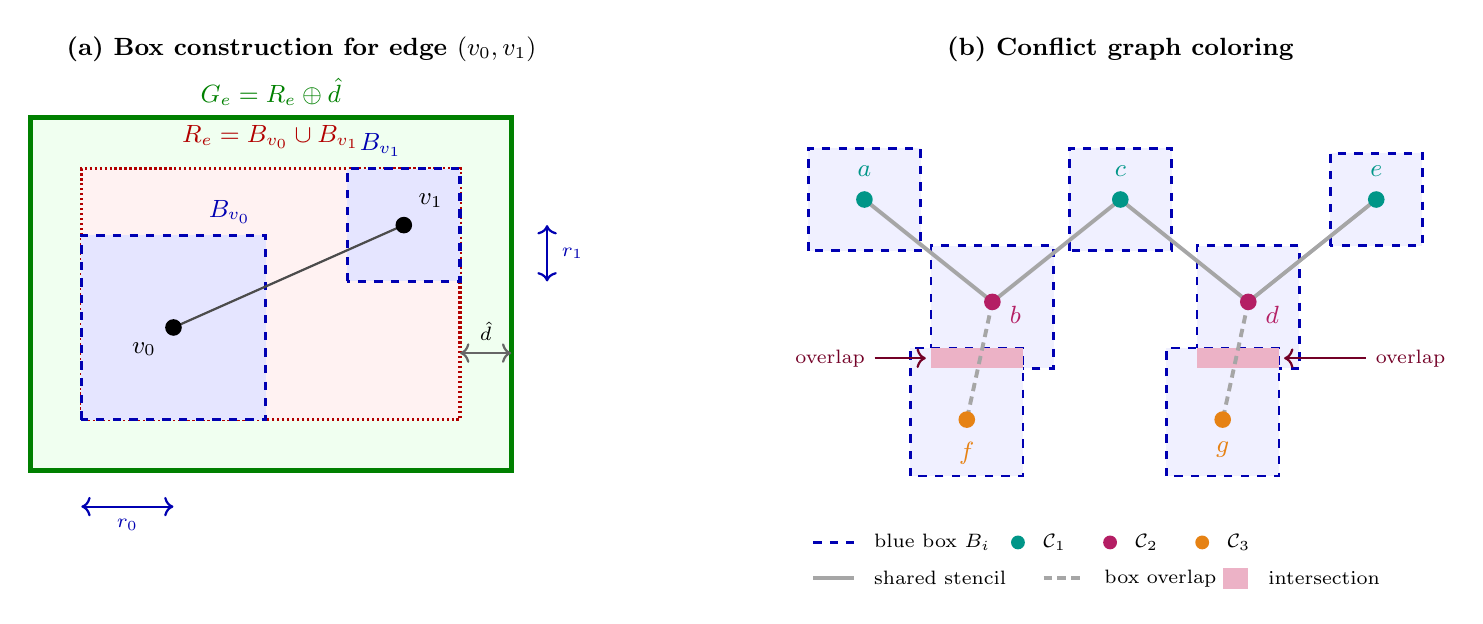
\begin{tikzpicture}[
  scale=0.65,
  every node/.style={font=\footnotesize},
  vert/.style={circle, inner sep=0pt, minimum size=6pt},
]

% ============ Left panel: box construction ============
\node[anchor=south, font=\small\bfseries] at (5.0,10.0)
  {(a) Box construction for edge $(v_0, v_1)$};

\coordinate (A) at (2.5, 5.0);
\coordinate (B) at (7.0, 7.0);

% Green box (outermost)
\fill[green!6] (-0.3, 2.2) rectangle (9.1, 9.1);
\draw[green!50!black, line width=1.8pt]
  (-0.3, 2.2) rectangle (9.1, 9.1);

% Red box
\fill[red!5] (0.7, 3.2) rectangle (8.1, 8.1);
\draw[red!70!black, thick, densely dotted, line width=1.2pt]
  (0.7, 3.2) rectangle (8.1, 8.1);

% Blue box A
\fill[blue!10] (0.7, 3.2) rectangle (4.3, 6.8);
\draw[blue!70!black, thick, dashed, line width=1.2pt]
  (0.7, 3.2) rectangle (4.3, 6.8);
\node[blue!70!black, font=\small, anchor=south east]
  at (4.2, 6.85) {$B_{v_0}$};

% Blue box B
\fill[blue!10] (5.9, 5.9) rectangle (8.1, 8.1);
\draw[blue!70!black, thick, dashed, line width=1.2pt]
  (5.9, 5.9) rectangle (8.1, 8.1);
\node[blue!70!black, font=\small, anchor=south west]
  at (5.95, 8.15) {$B_{v_1}$};

% Labels
\node[red!70!black, font=\small, anchor=south]
  at (4.4, 8.3) {$R_e = B_{v_0} \cup B_{v_1}$};
\node[green!50!black, font=\small, anchor=south]
  at (4.4, 9.15) {$G_e = R_e \oplus \hat{d}$};

% Edge
\draw[thick, black!70] (A) -- (B);

% Nodes
\node[vert, fill=black] at (A) {};
\node[anchor=north east, font=\small]
  at ($(A)+(-0.15,-0.1)$) {$v_0$};
\node[vert, fill=black] at (B) {};
\node[anchor=south west, font=\small]
  at ($(B)+(0.1,0.15)$) {$v_1$};

% r_0 arrow
\draw[<->, thick, blue!70!black]
  (0.7, 1.5) -- (2.5, 1.5);
\node[font=\scriptsize, blue!70!black, anchor=north]
  at (1.6, 1.45) {$r_0$};

% r_1 arrow
\draw[<->, thick, blue!70!black]
  (9.8, 5.9) -- (9.8, 7.0);
\node[font=\scriptsize, blue!70!black, anchor=west]
  at (9.9, 6.45) {$r_1$};

% d_hat arrow
\draw[<->, thick, black!60]
  (8.1, 4.5) -- (9.1, 4.5);
\node[font=\scriptsize, anchor=south] at (8.6, 4.55)
  {$\hat{d}$};

% ============ Right panel: coloring ============
\begin{scope}[xshift=14cm]

\node[anchor=south, font=\small\bfseries] at (7.0,10.0)
  {(b) Conflict graph coloring};

% Top chain
\coordinate (na) at (2.0, 7.5);
\coordinate (nb) at (4.5, 5.5);
\coordinate (nc) at (7.0, 7.5);
\coordinate (nd) at (9.5, 5.5);
\coordinate (ne) at (12.0, 7.5);

% Nearby nodes
\coordinate (nf) at (4.0, 3.2);
\coordinate (ng) at (9.0, 3.2);

% Overlap highlights (behind boxes)
\fill[purple!25] (3.3, 3.9) rectangle (5.1, 4.6);
\fill[purple!25] (8.4, 3.9) rectangle (10.1, 4.6);

% Blue boxes
% a
\fill[blue!6]
  ($(na)+(-1.1,-1.0)$) rectangle ($(na)+(1.1,1.0)$);
\draw[blue!70!black, thick, dashed, line width=1.0pt]
  ($(na)+(-1.1,-1.0)$) rectangle ($(na)+(1.1,1.0)$);

% b
\fill[blue!6]
  ($(nb)+(-1.2,-1.3)$) rectangle ($(nb)+(1.2,1.1)$);
\draw[blue!70!black, thick, dashed, line width=1.0pt]
  ($(nb)+(-1.2,-1.3)$) rectangle ($(nb)+(1.2,1.1)$);

% c
\fill[blue!6]
  ($(nc)+(-1.0,-1.0)$) rectangle ($(nc)+(1.0,1.0)$);
\draw[blue!70!black, thick, dashed, line width=1.0pt]
  ($(nc)+(-1.0,-1.0)$) rectangle ($(nc)+(1.0,1.0)$);

% d
\fill[blue!6]
  ($(nd)+(-1.0,-1.3)$) rectangle ($(nd)+(1.0,1.1)$);
\draw[blue!70!black, thick, dashed, line width=1.0pt]
  ($(nd)+(-1.0,-1.3)$) rectangle ($(nd)+(1.0,1.1)$);

% e
\fill[blue!6]
  ($(ne)+(-0.9,-0.9)$) rectangle ($(ne)+(0.9,0.9)$);
\draw[blue!70!black, thick, dashed, line width=1.0pt]
  ($(ne)+(-0.9,-0.9)$) rectangle ($(ne)+(0.9,0.9)$);

% f
\fill[blue!6]
  ($(nf)+(-1.1,-1.1)$) rectangle ($(nf)+(1.1,1.4)$);
\draw[blue!70!black, thick, dashed, line width=1.0pt]
  ($(nf)+(-1.1,-1.1)$) rectangle ($(nf)+(1.1,1.4)$);

% g
\fill[blue!6]
  ($(ng)+(-1.1,-1.1)$) rectangle ($(ng)+(1.1,1.4)$);
\draw[blue!70!black, thick, dashed, line width=1.0pt]
  ($(ng)+(-1.1,-1.1)$) rectangle ($(ng)+(1.1,1.4)$);

% Redraw overlap on top
\fill[purple!30] (3.3, 4.2) rectangle (5.1, 4.6);
\fill[purple!30] (8.5, 4.2) rectangle (10.1, 4.6);

% Mesh edges
\draw[thick, black!60] (na) -- (nb) -- (nc) -- (nd) -- (ne);

% Conflict edges: shared element
\draw[black!35, line width=1.4pt] (na) -- (nb);
\draw[black!35, line width=1.4pt] (nb) -- (nc);
\draw[black!35, line width=1.4pt] (nc) -- (nd);
\draw[black!35, line width=1.4pt] (nd) -- (ne);

% Conflict edges: box overlap
\draw[black!35, line width=1.4pt, densely dashed] (nb) -- (nf);
\draw[black!35, line width=1.4pt, densely dashed] (nd) -- (ng);

% Overlap annotations
\draw[->, purple!60!black, thick]
  (2.2, 4.4) -- (3.2, 4.4);
\node[font=\scriptsize, purple!60!black, anchor=east]
  at (2.2, 4.4) {overlap};

\draw[->, purple!60!black, thick]
  (11.8, 4.4) -- (10.2, 4.4);
\node[font=\scriptsize, purple!60!black, anchor=west]
  at (11.8, 4.4) {overlap};

% Node colors
\definecolor{c1color}{RGB}{0,150,136}
\definecolor{c2color}{RGB}{180,30,100}
\definecolor{c3color}{RGB}{230,130,20}

\node[vert, fill=c1color] at (na) {};
\node[anchor=south, c1color, font=\small]
  at ($(na)+(0,0.25)$) {$a$};

\node[vert, fill=c2color] at (nb) {};
\node[anchor=north west, c2color, font=\small]
  at ($(nb)+(0.15,0.1)$) {$b$};

\node[vert, fill=c1color] at (nc) {};
\node[anchor=south, c1color, font=\small]
  at ($(nc)+(0,0.25)$) {$c$};

\node[vert, fill=c2color] at (nd) {};
\node[anchor=north west, c2color, font=\small]
  at ($(nd)+(0.15,0.1)$) {$d$};

\node[vert, fill=c1color] at (ne) {};
\node[anchor=south, c1color, font=\small]
  at ($(ne)+(0,0.25)$) {$e$};

\node[vert, fill=c3color] at (nf) {};
\node[anchor=north, c3color, font=\small]
  at ($(nf)+(0,-0.25)$) {$f$};

\node[vert, fill=c3color] at (ng) {};
\node[anchor=north, c3color, font=\small]
  at ($(ng)+(0,-0.25)$) {$g$};

% Legend
\draw[blue!70!black, thick, dashed, line width=1.0pt]
  (1.0, 0.8) -- ++(0.8,0);
\node[anchor=west, font=\scriptsize] at (2.0, 0.8)
  {blue box $B_i$};

\node[vert, fill=c1color, minimum size=5pt]
  at (5.0, 0.8) {};
\node[anchor=west, font=\scriptsize] at (5.3, 0.8)
  {$\mathcal{C}_1$};
\node[vert, fill=c2color, minimum size=5pt]
  at (6.8, 0.8) {};
\node[anchor=west, font=\scriptsize] at (7.1, 0.8)
  {$\mathcal{C}_2$};
\node[vert, fill=c3color, minimum size=5pt]
  at (8.6, 0.8) {};
\node[anchor=west, font=\scriptsize] at (8.9, 0.8)
  {$\mathcal{C}_3$};

\draw[black!35, line width=1.4pt]
  (1.0, 0.1) -- ++(0.8,0);
\node[anchor=west, font=\scriptsize] at (2.0, 0.1)
  {shared stencil};
\draw[black!35, line width=1.4pt, densely dashed]
  (5.5, 0.1) -- ++(0.8,0);
\node[anchor=west, font=\scriptsize] at (6.5, 0.1)
  {box overlap};
\fill[purple!30] (9.0, -0.1) rectangle (9.5, 0.3);
\node[anchor=west, font=\scriptsize] at (9.7, 0.1)
  {intersection};

\end{scope}
\end{tikzpicture}
\caption{%
\textbf{(a)}~Box construction for edge $e=(v_0,v_1)$. Each node
receives an isotropic blue box~$B_{v_i}$ with half-width~$r_i$.
The red box~$R_e$ is the axis-aligned bounding box of
$B_{v_0}\cup B_{v_1}$. The green box
$G_e = R_e \oplus \hat{d}$ adds barrier-distance padding.
\textbf{(b)}~Conflict graph coloring. Dashed boxes are blue
boxes~$B_i$; node colors indicate batch assignment. Nodes
$a$--$e$ form a mesh chain; $f$ and $g$ belong to a nearby
region. Solid gray edges denote conflicts from shared stencils.
Dashed gray edges denote conflicts from overlapping blue boxes
(purple shading). Three colors suffice: $f$ and $g$ cannot join
$\mathcal{C}_2$ because their blue boxes overlap those of $b$
and~$d$, respectively.}
\label{fig:boxes}
\end{figure*}


\begin{figure*}[t]
\centering
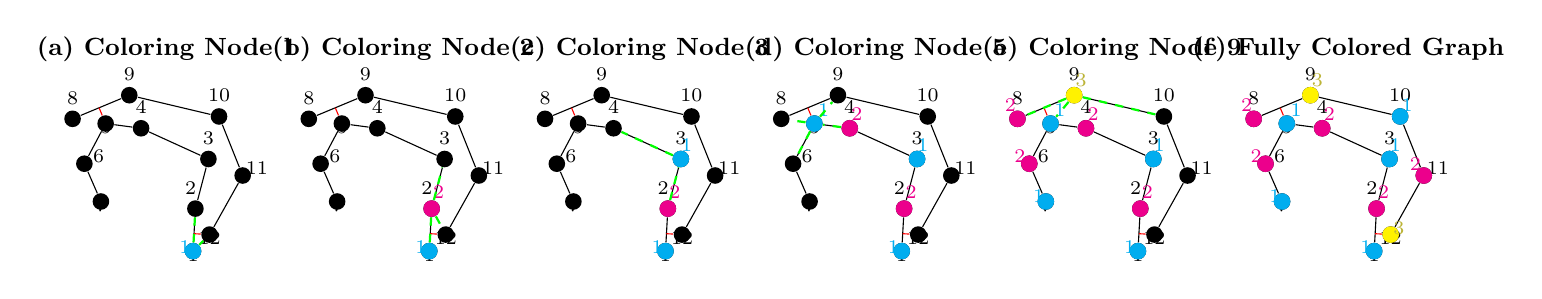
\begin{tikzpicture}[
  scale=0.3,
  every node/.style={font=\footnotesize},
  vert/.style={circle, inner sep=0pt, minimum size=6pt},
]

% ================== Top row: panels (a), (b), (c) ==================

\begin{scope}[xshift=0cm, yshift=0cm]
  \node[anchor=south, font=\small\bfseries] at (5.0,10.0) {(a) Coloring Node 1};

  % ================== Base Nodes ==================
  \node[vert, fill=black] (7a) at (2.2,4.5) {};
  \node[font=\scriptsize, anchor=south] at (2.2,3.65) {7};
  
  \node[vert, fill=black] (6a) at (1.5,6.1) {};
  \node[font=\scriptsize, anchor=south] at (2.1,5.75) {6};

  \node[vert, fill=black] (5a) at (2.4,7.8) {};
  \node[font=\scriptsize, anchor=south] at (2.4,6.95) {5};

  \node[vert, fill=black] (4a) at (3.9,7.6) {};
  \node[font=\scriptsize, anchor=south] at (3.9,7.8) {4};

  \node[vert, fill=black] (3a) at (6.75,6.3) {};
  \node[font=\scriptsize, anchor=south] at (6.75,6.5) {3};

  \node[vert, fill=black] (2a) at (6.2,4.2) {};
  \node[font=\scriptsize, anchor=south] at (6.0,4.4) {2};

  \node[vert, fill=black] (1a) at (6.1,2.4) {};
  \node[font=\scriptsize, anchor=south] at (6.1,1.55) {1};

  \node[vert, fill=black] (8a) at (1,8) {};
  \node[font=\scriptsize, anchor=south] at (1,8.2) {8};

  \node[vert, fill=black] (9a) at (3.4,9) {};
  \node[font=\scriptsize, anchor=south] at (3.4,9.2) {9};

  \node[vert, fill=black] (10a) at (7.2,8.1) {};
  \node[font=\scriptsize, anchor=south] at (7.2,8.3) {10};

  \node[vert, fill=black] (11a) at (8.2,5.6) {};
  \node[font=\scriptsize, anchor=south] at (8.8,5.25) {11};

  \node[vert, fill=black] (12a) at (6.8,3.1) {};
  \node[font=\scriptsize, anchor=south] at (6.8,2.25) {12};

  % ================== Base EDges ==================
  \draw (1a) -- (2a);
  \draw (2a) -- (3a);
  \draw (3a) -- (4a);
  \draw (4a) -- (5a);
  \draw (5a) -- (6a);
  \draw (6a) -- (7a);
  \draw (8a) -- (9a);
  \draw (9a) -- (10a);
  \draw (10a) -- (11a);
  \draw (11a) -- (12a);
  
  % ================== Base dhat ==================
  \draw[red] (12a) -- (6.141,3.137);
  \draw[red] (5a) -- (2.122,8.468);
  
  % ================== Coloring ==================
  \node[vert, fill=cyan] (1a) at (6.1,2.4) {};
  \node[font=\scriptsize, anchor=south, text=cyan] at (5.75,1.9) {1};

  \draw[dashed, green, thick] (1a) -- (2a);
  \draw[dashed, green, thick] (1a) -- (12a);


\end{scope}

\begin{scope}[xshift=10cm, yshift=0cm]
  \node[anchor=south, font=\small\bfseries] at (5.0,10.0) {(b) Coloring Node 2};

  % ================== Base Nodes ==================
  \node[vert, fill=black] (7b) at (2.2,4.5) {};
  \node[font=\scriptsize, anchor=south] at (2.2,3.65) {7};

  \node[vert, fill=black] (6b) at (1.5,6.1) {};
  \node[font=\scriptsize, anchor=south] at (2.1,5.75) {6};

  \node[vert, fill=black] (5b) at (2.4,7.8) {};
  \node[font=\scriptsize, anchor=south] at (2.4,6.95) {5};

  \node[vert, fill=black] (4b) at (3.9,7.6) {};
  \node[font=\scriptsize, anchor=south] at (3.9,7.8) {4};

  \node[vert, fill=black] (3b) at (6.75,6.3) {};
  \node[font=\scriptsize, anchor=south] at (6.75,6.5) {3};

  \node[vert, fill=black] (2b) at (6.2,4.2) {};
  \node[font=\scriptsize, anchor=south] at (6.0,4.4) {2};

  \node[vert, fill=black] (1b) at (6.1,2.4) {};
  \node[font=\scriptsize, anchor=south] at (6.1,1.55) {1};

  \node[vert, fill=black] (8b) at (1,8) {};
  \node[font=\scriptsize, anchor=south] at (1,8.2) {8};

  \node[vert, fill=black] (9b) at (3.4,9) {};
  \node[font=\scriptsize, anchor=south] at (3.4,9.2) {9};

  \node[vert, fill=black] (10b) at (7.2,8.1) {};
  \node[font=\scriptsize, anchor=south] at (7.2,8.3) {10};

  \node[vert, fill=black] (11b) at (8.2,5.6) {};
  \node[font=\scriptsize, anchor=south] at (8.8,5.25) {11};

  \node[vert, fill=black] (12b) at (6.8,3.1) {};
  \node[font=\scriptsize, anchor=south] at (6.8,2.25) {12};

  % ================== Base EDges ==================
  \draw (1b) -- (2b);
  \draw (2b) -- (3b);
  \draw (3b) -- (4b);
  \draw (4b) -- (5b);
  \draw (5b) -- (6b);
  \draw (6b) -- (7b);
  \draw (8b) -- (9b);
  \draw (9b) -- (10b);
  \draw (10b) -- (11b);
  \draw (11b) -- (12b);

  % ================== Base dhat ==================
  \draw[red] (12b) -- (6.141,3.137);
  \draw[red] (5b) -- (2.122,8.468);

  % ================== Coloring ==================
  \node[vert, fill=cyan] (1b) at (6.1,2.4) {};
  \node[font=\scriptsize, anchor=south, text=cyan] at (5.75,1.9) {1};
  \node[vert, fill=magenta] (2b) at (6.2,4.2) {};
  \node[font=\scriptsize, anchor=south, text=magenta] at (6.5,4.2) {2};

  \draw[dashed, green, thick] (1b) -- (2b);
  \draw[dashed, green, thick] (2b) -- (3b);
  \draw[dashed, green, thick] (2b) -- (12b);

\end{scope}

\begin{scope}[xshift=20cm, yshift=0cm]
  \node[anchor=south, font=\small\bfseries] at (5.0,10.0) {(c) Coloring Node 3};

  % ================== Base Nodes ==================
  \node[vert, fill=black] (7c) at (2.2,4.5) {};
  \node[font=\scriptsize, anchor=south] at (2.2,3.65) {7};
  
  \node[vert, fill=black] (6c) at (1.5,6.1) {};
  \node[font=\scriptsize, anchor=south] at (2.1,5.75) {6};

  \node[vert, fill=black] (5c) at (2.4,7.8) {};
  \node[font=\scriptsize, anchor=south] at (2.4,6.95) {5};

  \node[vert, fill=black] (4c) at (3.9,7.6) {};
  \node[font=\scriptsize, anchor=south] at (3.9,7.8) {4};

  \node[vert, fill=black] (3c) at (6.75,6.3) {};
  \node[font=\scriptsize, anchor=south] at (6.75,6.5) {3};

  \node[vert, fill=black] (2c) at (6.2,4.2) {};
  \node[font=\scriptsize, anchor=south] at (6.0,4.4) {2};

  \node[vert, fill=black] (1c) at (6.1,2.4) {};
  \node[font=\scriptsize, anchor=south] at (6.1,1.55) {1};

  \node[vert, fill=black] (8c) at (1,8) {};
  \node[font=\scriptsize, anchor=south] at (1,8.2) {8};

  \node[vert, fill=black] (9c) at (3.4,9) {};
  \node[font=\scriptsize, anchor=south] at (3.4,9.2) {9};

  \node[vert, fill=black] (10c) at (7.2,8.1) {};
  \node[font=\scriptsize, anchor=south] at (7.2,8.3) {10};

  \node[vert, fill=black] (11c) at (8.2,5.6) {};
  \node[font=\scriptsize, anchor=south] at (8.8,5.25) {11};

  \node[vert, fill=black] (12c) at (6.8,3.1) {};
  \node[font=\scriptsize, anchor=south] at (6.8,2.25) {12};

  % ================== Base EDges ==================
  \draw (1c) -- (2c);
  \draw (2c) -- (3c);
  \draw (3c) -- (4c);
  \draw (4c) -- (5c);
  \draw (5c) -- (6c);
  \draw (6c) -- (7c);
  \draw (8c) -- (9c);
  \draw (9c) -- (10c);
  \draw (10c) -- (11c);
  \draw (11c) -- (12c);
  
  % ================== Base dhat ==================
  \draw[red] (12c) -- (6.141,3.137);
  \draw[red] (5c) -- (2.122,8.468);

% ================== Coloring ==================
  \node[vert, fill=cyan] (1c) at (6.1,2.4) {};
  \node[font=\scriptsize, anchor=south, text=cyan] at (5.75,1.9) {1};
  \node[vert, fill=magenta] (2c) at (6.2,4.2) {};
  \node[font=\scriptsize, anchor=south, text=magenta] at (6.5,4.2) {2};
  \node[vert, fill=cyan] (3c) at (6.75,6.3) {};
  \node[font=\scriptsize, anchor=south, text=cyan] at (7,6.2) {1};

  \draw[dashed, green, thick] (2c) -- (3c);
  \draw[dashed, green, thick] (3c) -- (4c);

\end{scope}

% ================== Bottom row: panels (d), (e), (f) ==================
\begin{scope}[xshift=30cm, yshift=0cm]
  \node[anchor=south, font=\small\bfseries] at (5.0,10.0) {(d) Coloring Node 5};

  % ================== Base Nodes ==================
  \node[vert, fill=black] (7d) at (2.2,4.5) {};
  \node[font=\scriptsize, anchor=south] at (2.2,3.65) {7};
  
  \node[vert, fill=black] (6d) at (1.5,6.1) {};
  \node[font=\scriptsize, anchor=south] at (2.1,5.75) {6};

  \node[vert, fill=black] (5d) at (2.4,7.8) {};
  \node[font=\scriptsize, anchor=south] at (2.4,6.95) {5};

  \node[vert, fill=black] (4d) at (3.9,7.6) {};
  \node[font=\scriptsize, anchor=south] at (3.9,7.8) {4};

  \node[vert, fill=black] (3d) at (6.75,6.3) {};
  \node[font=\scriptsize, anchor=south] at (6.75,6.5) {3};

  \node[vert, fill=black] (2d) at (6.2,4.2) {};
  \node[font=\scriptsize, anchor=south] at (6.0,4.4) {2};

  \node[vert, fill=black] (1d) at (6.1,2.4) {};
  \node[font=\scriptsize, anchor=south] at (6.1,1.55) {1};

  \node[vert, fill=black] (8d) at (1,8) {};
  \node[font=\scriptsize, anchor=south] at (1,8.2) {8};

  \node[vert, fill=black] (9d) at (3.4,9) {};
  \node[font=\scriptsize, anchor=south] at (3.4,9.2) {9};

  \node[vert, fill=black] (10d) at (7.2,8.1) {};
  \node[font=\scriptsize, anchor=south] at (7.2,8.3) {10};

  \node[vert, fill=black] (11d) at (8.2,5.6) {};
  \node[font=\scriptsize, anchor=south] at (8.8,5.25) {11};

  \node[vert, fill=black] (12d) at (6.8,3.1) {};
  \node[font=\scriptsize, anchor=south] at (6.8,2.25) {12};

  % ================== Base EDges ==================
  \draw (1d) -- (2d);
  \draw (2d) -- (3d);
  \draw (3d) -- (4d);
  \draw (4d) -- (5d);
  \draw (5d) -- (6d);
  \draw (6d) -- (7d);
  \draw (8d) -- (9d);
  \draw (9d) -- (10d);
  \draw (10d) -- (11d);
  \draw (11d) -- (12d);
  
  % ================== Base dhat ==================
  \draw[red] (12d) -- (6.141,3.137);
  \draw[red] (5d) -- (2.122,8.468);

  % ================== Coloring ==================
  \node[vert, fill=cyan] (1d) at (6.1,2.4) {};
  \node[font=\scriptsize, anchor=south, text=cyan] at (5.75,1.9) {1};
  \node[vert, fill=magenta] (2d) at (6.2,4.2) {};
  \node[font=\scriptsize, anchor=south, text=magenta] at (6.5,4.2) {2};
  \node[vert, fill=cyan] (3d) at (6.75,6.3) {};
  \node[font=\scriptsize, anchor=south, text=cyan] at (7,6.2) {1};
  \node[vert, fill=magenta] (4d) at (3.9,7.6) {};
  \node[font=\scriptsize, anchor=south, text=magenta] at (4.2,7.5) {2};
  \node[vert, fill=cyan] (5d) at (2.4,7.8) {};
  \node[font=\scriptsize, anchor=south, text=cyan] at (2.8,7.7) {1};
  
  \draw[dashed, green, thick] (4d) -- (5d);
  \draw[dashed, green, thick] (5d) -- (6d);
  \draw[dashed, green, thick] (5d) -- (8d);
  \draw[dashed, green, thick] (5d) -- (9d);


\end{scope}

\begin{scope}[xshift=40cm, yshift=0cm]
  \node[anchor=south, font=\small\bfseries] at (5.0,10.0) {(e) Coloring Node 9};

  % ================== Base Nodes ==================
  \node[vert, fill=black] (7e) at (2.2,4.5) {};
  \node[font=\scriptsize, anchor=south] at (2.2,3.65) {7};
  
  \node[vert, fill=black] (6e) at (1.5,6.1) {};
  \node[font=\scriptsize, anchor=south] at (2.1,5.75) {6};

  \node[vert, fill=black] (5e) at (2.4,7.8) {};
  \node[font=\scriptsize, anchor=south] at (2.4,6.95) {5};

  \node[vert, fill=black] (4e) at (3.9,7.6) {};
  \node[font=\scriptsize, anchor=south] at (3.9,7.8) {4};

  \node[vert, fill=black] (3e) at (6.75,6.3) {};
  \node[font=\scriptsize, anchor=south] at (6.75,6.5) {3};

  \node[vert, fill=black] (2e) at (6.2,4.2) {};
  \node[font=\scriptsize, anchor=south] at (6.0,4.4) {2};

  \node[vert, fill=black] (1e) at (6.1,2.4) {};
  \node[font=\scriptsize, anchor=south] at (6.1,1.55) {1};

  \node[vert, fill=black] (8e) at (1,8) {};
  \node[font=\scriptsize, anchor=south] at (1,8.2) {8};

  \node[vert, fill=black] (9e) at (3.4,9) {};
  \node[font=\scriptsize, anchor=south] at (3.4,9.2) {9};

  \node[vert, fill=black] (10e) at (7.2,8.1) {};
  \node[font=\scriptsize, anchor=south] at (7.2,8.3) {10};

  \node[vert, fill=black] (11e) at (8.2,5.6) {};
  \node[font=\scriptsize, anchor=south] at (8.8,5.25) {11};

  \node[vert, fill=black] (12e) at (6.8,3.1) {};
  \node[font=\scriptsize, anchor=south] at (6.8,2.25) {12};

  % ================== Base EDges ==================
  \draw (1e) -- (2e);
  \draw (2e) -- (3e);
  \draw (3e) -- (4e);
  \draw (4e) -- (5e);
  \draw (5e) -- (6e);
  \draw (6e) -- (7e);
  \draw (8e) -- (9e);
  \draw (9e) -- (10e);
  \draw (10e) -- (11e);
  \draw (11e) -- (12e);
  
  % ================== Base dhat ==================
  \draw[red] (12e) -- (6.141,3.137);
  \draw[red] (5e) -- (2.122,8.468);

% ================== Coloring ==================
  \node[vert, fill=cyan] (1e) at (6.1,2.4) {};
  \node[font=\scriptsize, anchor=south, text=cyan] at (5.75,1.9) {1};
  \node[vert, fill=magenta] (2e) at (6.2,4.2) {};
  \node[font=\scriptsize, anchor=south, text=magenta] at (6.5,4.2) {2};
  \node[vert, fill=cyan] (3e) at (6.75,6.3) {};
  \node[font=\scriptsize, anchor=south, text=cyan] at (7,6.2) {1};
  \node[vert, fill=magenta] (4e) at (3.9,7.6) {};
  \node[font=\scriptsize, anchor=south, text=magenta] at (4.2,7.5) {2};
  \node[vert, fill=cyan] (5e) at (2.4,7.8) {};
  \node[font=\scriptsize, anchor=south, text=cyan] at (2.8,7.7) {1};
  
  \node[vert, fill=magenta] (6e) at (1.5,6.1) {};
  \node[font=\scriptsize, anchor=south, text=magenta] at (1.1,5.75) {2};
  \node[vert, fill=cyan] (7e) at (2.2,4.5) {};
  \node[font=\scriptsize, anchor=south, text=cyan] at (1.9,4.05) {1};
  \node[vert, fill=magenta] (8e) at (1,8) {};
  \node[font=\scriptsize, anchor=south, text=magenta] at (0.7,7.9) {2};
  \node[vert, fill=yellow] (9e) at (3.4,9) {};
  \node[font=\scriptsize, anchor=south,text=yellow!70!black] at (3.7,8.95) {3};
  
  \draw[dashed, green, thick] (9e) -- (5e);
  \draw[dashed, green, thick] (9e) -- (8e);
  \draw[dashed, green, thick] (9e) -- (10e);



\end{scope}

\begin{scope}[xshift=50cm, yshift=0cm]
  \node[anchor=south, font=\small\bfseries] at (5.0,10.0) {(f) Fully Colored Graph};

  % ================== Base Nodes ==================
  \node[vert, fill=black] (7f) at (2.2,4.5) {};
  \node[font=\scriptsize, anchor=south] at (2.2,3.65) {7};
  
  \node[vert, fill=black] (6f) at (1.5,6.1) {};
  \node[font=\scriptsize, anchor=south] at (2.1,5.75) {6};

  \node[vert, fill=black] (5f) at (2.4,7.8) {};
  \node[font=\scriptsize, anchor=south] at (2.4,6.95) {5};

  \node[vert, fill=black] (4f) at (3.9,7.6) {};
  \node[font=\scriptsize, anchor=south] at (3.9,7.8) {4};

  \node[vert, fill=black] (3f) at (6.75,6.3) {};
  \node[font=\scriptsize, anchor=south] at (6.75,6.5) {3};

  \node[vert, fill=black] (2f) at (6.2,4.2) {};
  \node[font=\scriptsize, anchor=south] at (6.0,4.4) {2};

  \node[vert, fill=black] (1f) at (6.1,2.4) {};
  \node[font=\scriptsize, anchor=south] at (6.1,1.55) {1};

  \node[vert, fill=black] (8f) at (1,8) {};
  \node[font=\scriptsize, anchor=south] at (1,8.2) {8};

  \node[vert, fill=black] (9f) at (3.4,9) {};
  \node[font=\scriptsize, anchor=south] at (3.4,9.2) {9};

  \node[vert, fill=black] (10f) at (7.2,8.1) {};
  \node[font=\scriptsize, anchor=south] at (7.2,8.3) {10};

  \node[vert, fill=black] (11f) at (8.2,5.6) {};
  \node[font=\scriptsize, anchor=south] at (8.8,5.25) {11};

  \node[vert, fill=black] (12f) at (6.8,3.1) {};
  \node[font=\scriptsize, anchor=south] at (6.8,2.25) {12};

  % ================== Base EDges ==================
  \draw (1f) -- (2f);
  \draw (2f) -- (3f);
  \draw (3f) -- (4f);
  \draw (4f) -- (5f);
  \draw (5f) -- (6f);
  \draw (6f) -- (7f);
  \draw (8f) -- (9f);
  \draw (9f) -- (10f);
  \draw (10f) -- (11f);
  \draw (11f) -- (12f);
  
  % ================== Base dhat ==================
  \draw[red] (12f) -- (6.141,3.137);
  \draw[red] (5f) -- (2.122,8.468);

  % ================== Coloring ==================
  \node[vert, fill=cyan] (1f) at (6.1,2.4) {};
  \node[font=\scriptsize, anchor=south, text=cyan] at (5.75,1.9) {1};
  \node[vert, fill=magenta] (2f) at (6.2,4.2) {};
  \node[font=\scriptsize, anchor=south, text=magenta] at (6.5,4.2) {2};
  \node[vert, fill=cyan] (3f) at (6.75,6.3) {};
  \node[font=\scriptsize, anchor=south, text=cyan] at (7,6.2) {1};
  \node[vert, fill=magenta] (4f) at (3.9,7.6) {};
  \node[font=\scriptsize, anchor=south, text=magenta] at (4.2,7.5) {2};
  \node[vert, fill=cyan] (5f) at (2.4,7.8) {};
  \node[font=\scriptsize, anchor=south, text=cyan] at (2.8,7.7) {1};
  \node[vert, fill=magenta] (6f) at (1.5,6.1) {};
  \node[font=\scriptsize, anchor=south, text=magenta] at (1.1,5.75) {2};
  \node[vert, fill=cyan] (7f) at (2.2,4.5) {};
  \node[font=\scriptsize, anchor=south, text=cyan] at (1.9,4.05) {1};
  \node[vert, fill=magenta] (8f) at (1,8) {};
  \node[font=\scriptsize, anchor=south, text=magenta] at (0.7,7.9) {2};
  \node[vert, fill=yellow] (9f) at (3.4,9) {};
  \node[font=\scriptsize, anchor=south,text=yellow!70!black] at (3.7,8.95) {3};
  
  \node[vert, fill=cyan] (10f) at (7.2,8.1) {};
  \node[font=\scriptsize, anchor=south, text=cyan] at (7.5,7.9) {1};
  \node[vert, fill=magenta] (11f) at (8.2,5.6) {};
  \node[font=\scriptsize, anchor=south, text =magenta] at (7.85,5.4) {2};
  \node[vert, fill=yellow] (12f) at (6.8,3.1) {};
  \node[font=\scriptsize, anchor=south, text=yellow!70!black] at (7.15,2.7) {3};


\end{scope}

\end{tikzpicture}
\caption{%
\textbf~TODO: description of graph features
\textbf{(a)}~description of a
\textbf{(b)}~
\textbf{(c)}~
\textbf{(d)}~
\textbf{(e)}~
\textbf{(f)}~description of f
}
\label{fig:boxes}
\end{figure*}

\end{document}
